\documentclass[11pt]{amsart}
\usepackage{geometry}                % See geometry.pdf to learn the layout options. There are lots.
\geometry{letterpaper}                   % ... or a4paper or a5paper or ... 
%\geometry{landscape}                % Activate for for rotated page geometry
%\usepackage[parfill]{parskip}    % Activate to begin paragraphs with an empty line rather than an indent
\usepackage{graphicx}
\usepackage{amssymb}
\usepackage{epstopdf}
\usepackage [autostyle, english = american]{csquotes}
\usepackage{hyperref}
\MakeOuterQuote{"}
\DeclareGraphicsRule{.tif}{png}{.png}{`convert #1 `dirname #1`/`basename #1 .tif`.png}

\title{Project 7: Solving A System of Differential Equations Numerically}
%\author{Jessica Bartley}
%\date{}                                           % Activate to display a given date or no date

\begin{document}
\maketitle
%\section{}
%\subsection{}

In this project we will simulate the orbit of a comet within an earth's central gravitational potential.  The data to compute are $r$, $\dot r$, $\phi$, and $\dot \phi$ as functions of time.  The comet moves in a plane that intersects the Earth-Sun orbital plane as in Figure 1 and worked out in more detail in Figure 2.  Our $r$ and $\phi$ are measured in the comet's plane of motion, and this is the path we aim to graph.
\newline

The geometry of this problem is somewhat complex.  Our given initial conditions are measured from the Earth - Sun plane (Figure 1 green / Figure 2 black ) but we are instructed to graph the comet as it travels through the Comet - Sun plane (Figure 1 blue / Figure 2 red).  In order to work in this Comet - Sun plane we must transform all vectors by use of a rotation matrix about the z and y axes.

\begin{figure}[ht!]
\centering
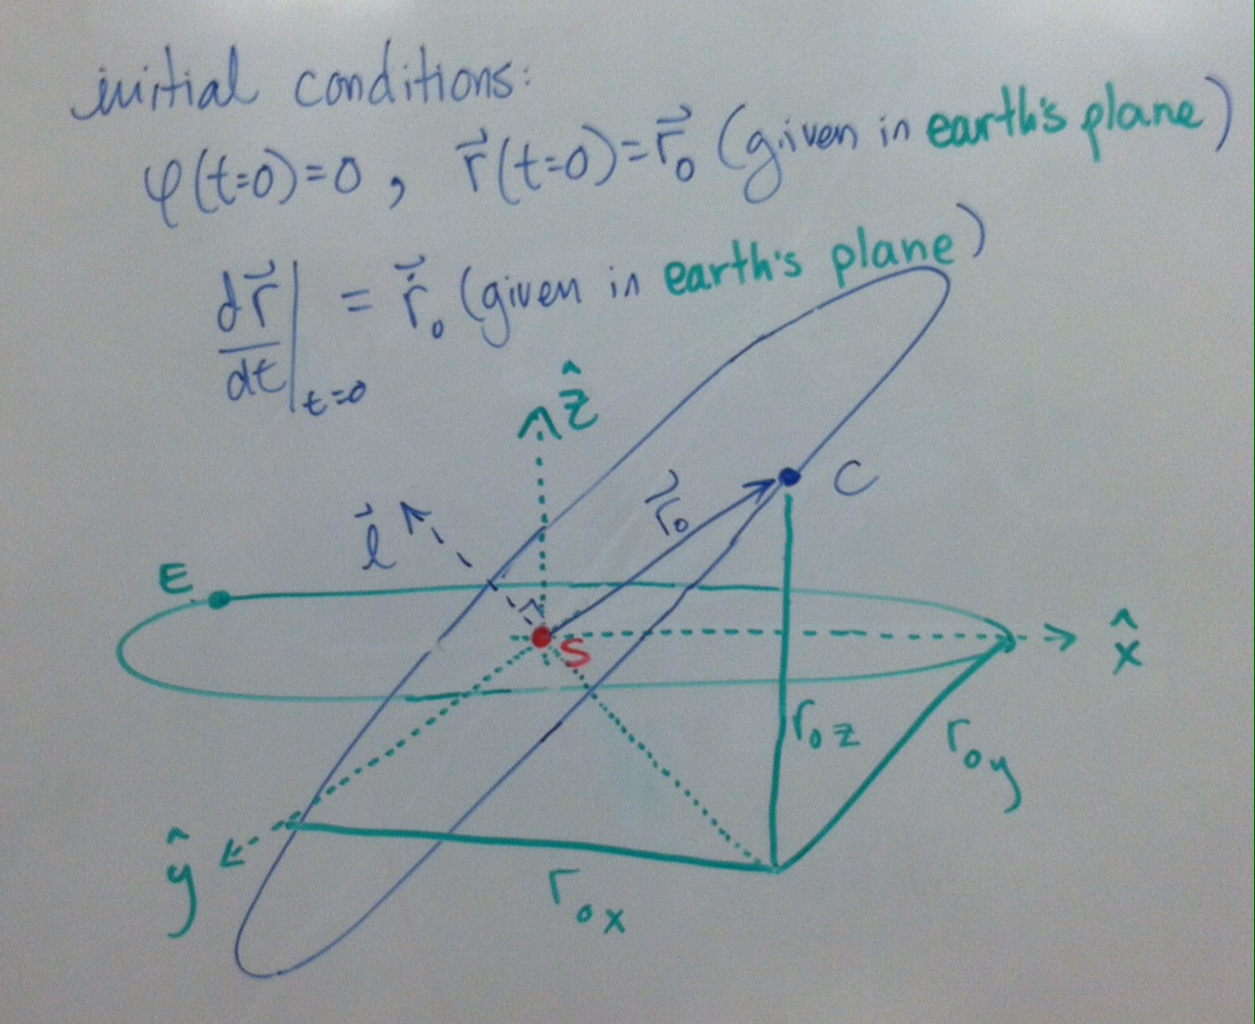
\includegraphics[width=110mm]{Orbit.jpg}
\caption{Coordinate system set up for this problem}
\label{overflow}
\end{figure}

\begin{figure}[ht!]
\centering
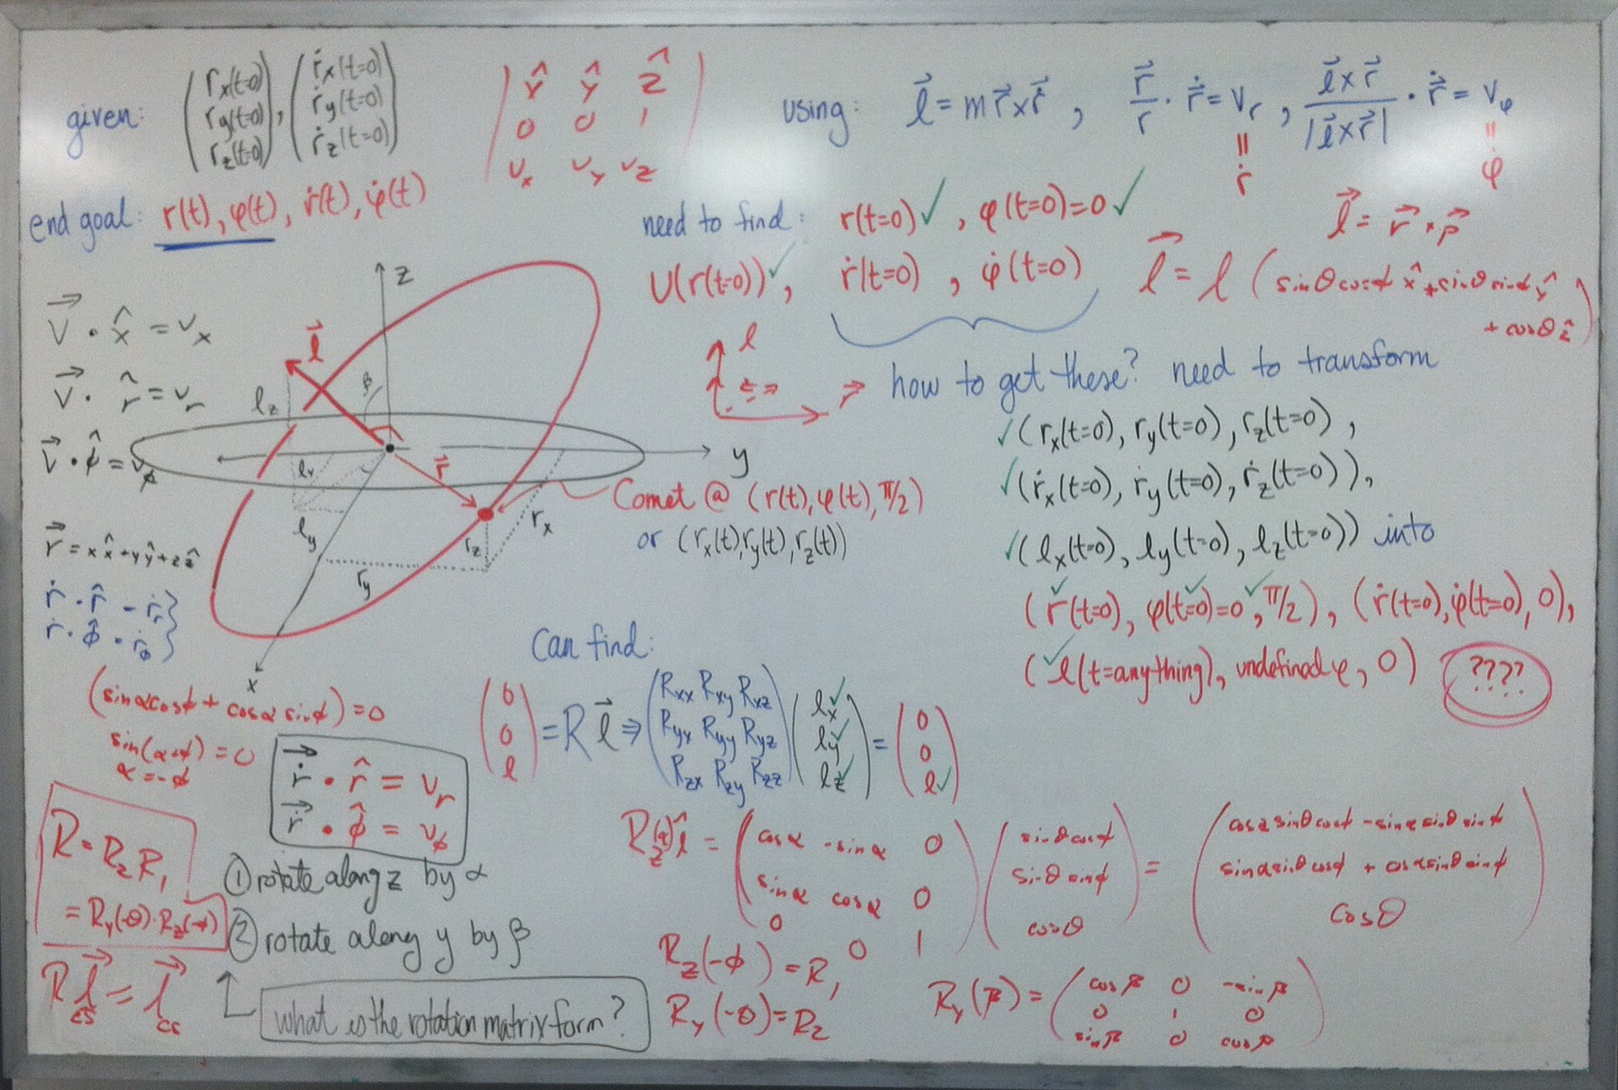
\includegraphics[width=150mm]{fig2.jpg}
\caption{Coordinate system set up for this problem}
\label{overflow}
\end{figure}

First I will explain the physics, then I will talk about how I approached the code.  Conservation laws give that the magnitude of the angular momentum does not change over time.  Further, the angular momentum vector $\bold l = m \bold r \times \bold{\dot r}$, is always perpendicular to the comet's plane of motion (note, the dot indicates a time derivative.)  In this sense, solving for the angular momentum vector in the Earth - Sun plane tells us how tilted the two planes are with respect to each other.  Our first aim is the find this $\bold l$ tilt, and then transform the vector so that it aligns with the z-axis.  Once we have the transformation matrix, we can apply it to the given initial conditions so that all vectors are in the desired Comet - Sun plane.
\newline

After we transform all vectors into the correct plane we can calculate the radial and angular velocities:

\begin{align}
  \frac{\bold r}{r} \cdot \bold{\dot r} &= v_r & \frac{\bold l \times \bold r}{| \bold l \times \bold r |} \cdot \bold{\dot r} &= v_\phi
\end{align}
\vspace{2 mm}

We then use these as initial conditions into our set of four coupled differential equations describing the motion of the comet.  For convenience we set the comet's mass to $m_{comet}=1 \ll m_{sun}$ (and thus the reduced mass becomes $\frac{m_{comet} m_{sun}} {m_{comet} + m_{sun}} \approx \frac{m_{sun}} { m_{sun}} = 1$) then our differential equations are expressed as:

\begin{align}
  \frac{dr}{dt} &= v_r
 &
  \frac{d v_r}{dt} &= - \frac{d U}{dr}
\end{align}

\begin{align}
 \frac{d \phi}{dt} &= \frac{v_{\phi}}{r^2}
 &  \frac{d v_{\phi} }{dt} &= 0
\end{align}
\vspace{2 mm}

The potential and its derivative are given by:

\begin{equation}
U = \frac{l^2}{2 r^2} - \frac{Gm_{sun}}{r} 
\end{equation}
\begin{equation}
\frac{d U}{d t} = - \frac{2l^2}{2 r^3} + \frac{Gm_{sun}}{r^2}
\end{equation}
\vspace{2 mm}

The initial conditions measured in AU and AU / dar respectively, as given in the Earth-Sun plane are:

\[
\bold r = 
  \begin{pmatrix} 0.3170787 \\ -1.887907 \\ 0.2396305 \end{pmatrix}
\]

\[
\bold{\dot r} = 
  \begin{pmatrix} 0.008180196 \\ 0.01188029 \\ 0.0006081217 \end{pmatrix}
\]
\vspace{2 mm}
\vspace{2 mm}

\textbf{The end goal of this project is to make a plot of $r$ vs $\phi$ which will show the comets' orbital path.}
\newline

\vspace{3 mm}

The steps for the code include:
\begin{enumerate}
\item Input the initial conditions.  
\item Write a function to transform vectors calculated in the Earth - Sun plane to the Comet - Sun plane and convert the vectors $l$, $\bold{r}(t=0)$ and $\bold{\dot r}(t=0)$.
\item Calculate the initial radial and angular velocities in the Comet - Sun plane.
\item Use the built in python "odeint" function to solve the system of four coupled differential equations and plot the results.
\end{enumerate}

Note: I have found an example python code that uses odeint to solve a system of four coupled differential equations.  I have uploaded it with my code.  The sample code works but mine does not.  I believe I am using the odeint module as per its documentation, but I am not getting the results I should have.

\end{document}  